\chapter{Lecture 1: The Theoretical Minimum}

These companion notes follow Leonard Susskind's opening lecture on quantum mechanics in the order in which the argument is actually built. A few retained board frames from the recorded lecture are kept as visual evidence, with credit to Leonard Susskind, LazyingArt LLC, and Video2Book. The point of departure is classical mechanics: a closed system, a state, and a deterministic rule for updating that state. The point of arrival, for this first lecture, is not yet a full quantum formalism, but the realization that the quantum space of states is not a set of classical alternatives. It is a complex vector space, and the odd behavior of qubits will have to be represented there.

\section{From Classical States to Quantum Abstraction}

The lecture begins by rebuilding classical mechanics from the ground up. First we have a system: an isolated thing whose history we wish to predict. Next we have a state: whatever data are needed, at a given instant, to predict the future. Finally we have equations of motion: rules that tell us how to update the state from one time to the next.

For a very simple system, such as an abstract coin, the update rules can be written almost insultingly plainly. One possible law of motion is that nothing happens:
\begin{align}
H &\mapsto H, &
T &\mapsto T.
\end{align}
Another possible law is alternation:
\begin{align}
H &\mapsto T, &
T &\mapsto H.
\end{align}
The point of these toy examples is not their content. It is the form. Classical mechanics is the business of updating a state:
\begin{equation}
s(t)\longmapsto s(t+\Delta t),
\end{equation}
and the update is deterministic once the state is known.

As we pass from discrete systems to continuous motion, the state space becomes larger and more abstract, but the basic classical idea does not change. One still imagines a system as carrying a definite state, and one still expects equations that carry that state forward in time.

At exactly this point the lecture inserts an important warning. Once physics leaves the range of ordinary experience, visualization becomes unreliable. We are not equipped to picture five-dimensional space, or even truly two-dimensional curved space without secretly embedding it in something larger. The remedy is not stronger pictorial intuition. The remedy is abstraction. We learn to manipulate symbols correctly, and only later do we acquire a new, more mathematical intuition.

\begin{remark}
This warning is structural, not rhetorical. The lecture is preparing us for the claim that quantum mechanics cannot be understood as a slightly exotic version of classical picture-thinking. If we insist on visualizing first and abstracting later, we will almost surely import the wrong logic.
\end{remark}

\section{Classical State Spaces and Classical Logic}

For classical systems, the state space is a set. That is the last stable classical foothold before the quantum break.

For an abstract coin,
\begin{equation}
\mathcal{S}_{\mathrm{coin}}=\{H,T\}.
\end{equation}
For an abstract die,
\begin{equation}
\mathcal{S}_{\mathrm{die}}=\{1,2,3,4,5,6\}.
\end{equation}
For a point particle moving along a line, the state is not just position but position together with momentum. The classical state space is phase space:
\begin{equation}
\mathcal{S}_{\mathrm{particle}}=\{(q,p)\mid q,p\in\mathbb{R}\}.
\end{equation}
In the first two examples the state space is a finite set; in the last it is a continuously infinite set. But in all cases it is still a set.

Once the state space is a set, propositions become subsets of that set. This is the origin of classical logical operations inside physics. If \(P\) and \(Q\) are propositions, then
\begin{equation}
P\wedge Q \leftrightarrow P\cap Q,
\qquad
P\vee Q \leftrightarrow P\cup Q,
\end{equation}
where the \( \vee \) here is the inclusive ``or.''

The die example makes the point cleanly. Let
\begin{align}
P_{\mathrm{odd}} &= \{1,3,5\},\\
Q_{\leq 3} &= \{1,2,3\}.
\end{align}
Then
\begin{align}
P_{\mathrm{odd}}\cap Q_{\leq 3} &= \{1,3\},\\
P_{\mathrm{odd}}\cup Q_{\leq 3} &= \{1,2,3,5\}.
\end{align}
So ``odd and less than or equal to three'' means intersection, while ``odd or less than or equal to three'' means union. Non-overlapping propositions have empty intersection; that is what it means for the classical ``and'' statement to be false.

This is the logic of set theory, and classical mechanics inherits it because classical state spaces are sets. The lecture then makes the decisive move: quantum mechanics does not. The state of a quantum system is not a point in a set of classical alternatives. In this first lecture we are told, before it is explained in detail, that the appropriate structure is a vector space.

\section{The Qubit, Its Notations, and the Apparatus}

Before discussing that vector space abstractly, the lecture returns to experiment and introduces the simplest quantum system: the qubit. It is the quantum analogue of the classical bit, and therefore the quantum analogue of the coin. But it is already clear that the analogy will not be exact.

The qubit is introduced first with familiar language, heads and tails, and then with a more useful two-valued variable \(\sigma\):
\begin{equation}
\sigma\in\{+1,-1\}.
\end{equation}
The three equivalent notational systems are
\begin{equation}
H \leftrightarrow \sigma=+1 \leftrightarrow \uparrow,
\qquad
T \leftrightarrow \sigma=-1 \leftrightarrow \downarrow.
\end{equation}
At this stage the arrows are explicitly only notation. They are not yet a claim that the qubit is literally an ordinary spatial vector.

\begin{figure}[ht]
\centering

\includegraphics[width=0.72\textwidth]{lecture_01_figure_02.png}
\caption{Qubit labels \(\sigma=\pm1\) and up/down notation.}
\end{figure}

The next ingredient is the apparatus, denoted \(A\). It is treated operationally as a black box with an orientation, a sensor, and a display window. In its neutral state the display is blank. When brought into interaction with the qubit, a faithful apparatus records one of only two outcomes:
\begin{equation}
\text{readout}\in\{+1,-1\}.
\end{equation}
The important point is not hidden mechanics inside the box, but what repeated use of the box reveals.

Suppose the first measurement gives \(+1\). Reset the apparatus to its blank state, bring it back immediately in the same orientation, and measure again. If nothing has happened to the qubit in the meantime, the result is confirmed. Repetition in the same orientation keeps the same answer:
\begin{equation}
+1\to +1\to +1\to \cdots,
\qquad
-1\to -1\to -1\to \cdots.
\end{equation}
Thus the first measurement is not merely a readout. It also prepares the qubit in the state corresponding to that readout. This is already a characteristic quantum theme: measurement and state-preparation are not separate acts.

The lecture then makes the next move. Prepare a qubit in the state \(\sigma=+1\), or in the arrow notation \(\uparrow\). Now turn the detector upside down. The readout flips sign. Turn the detector upright again and the sign flips back. So the up/down notation begins to acquire real physical content. This qubit does carry spatial directionality of some sort.

\section{Rotated Detectors and the Failure of the Classical Picture}

Once the detector has an orientation, a classical temptation immediately appears. Perhaps the qubit really is an ordinary vector in space, and perhaps the detector simply measures its component along the detector axis. For an upright detector this would fit the observed \(+1\). For an upside-down detector it would fit the observed \(-1\). So far the classical picture seems to survive.

\begin{figure}[ht]
\centering

\includegraphics[width=0.78\textwidth]{lecture_01_figure_03.png}
\caption{Prepared upward state with upright and sideways analyzer sketches.}
\end{figure}

But the lecture is designed to break exactly that intuition. After preparing the qubit ``up,'' we turn the detector sideways by \(90^\circ\). If the qubit were an ordinary classical pointer, its horizontal component would be zero. The classical answer would therefore be zero.

That is not what happens.

\begin{figure}[ht]
\centering
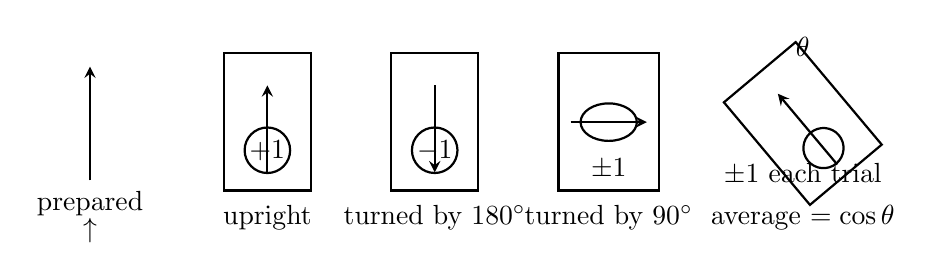
\begin{tikzpicture}[>=stealth,thick,scale=0.85]
\draw[->] (0,0)--(0,1.7);
\node at (0,-0.35) {prepared};
\node at (0,-0.75) {\(\uparrow\)};

\draw (2.0,-0.15) rectangle (3.3,1.9);
\draw (2.65,0.45) circle (0.34);
\draw[->] (2.65,0.12)--(2.65,1.42);
\node at (2.65,0.45) {\(+1\)};
\node at (2.65,-0.55) {upright};

\draw (4.5,-0.15) rectangle (5.8,1.9);
\draw (5.15,0.45) circle (0.34);
\draw[->] (5.15,1.42)--(5.15,0.12);
\node at (5.15,0.45) {\(-1\)};
\node at (5.15,-0.55) {turned by \(180^\circ\)};

\draw (7.0,-0.15) rectangle (8.5,1.9);
\draw (7.75,0.87) ellipse (0.42 and 0.28);
\draw[->] (7.18,0.87)--(8.32,0.87);
\node at (7.75,0.18) {\(\pm 1\)};
\node at (7.75,-0.55) {turned by \(90^\circ\)};

\begin{scope}[shift={(10.65,0.85)},rotate=40]
\draw (-0.7,-1.0) rectangle (0.7,1.0);
\draw (0,-0.48) circle (0.30);
\draw[->] (0,-0.80)--(0,0.58);
\end{scope}
\node at (10.65,0.10) {\(\pm 1\) each trial};
\node at (10.65,-0.55) {average \(=\cos\theta\)};
\node at (10.65,2.0) {\(\theta\)};
\end{tikzpicture}
\caption{Cleaned reconstruction of the detector-orientation experiments. The geometry follows the lecture's logic rather than every literal chalk arrow.}
\end{figure}

\subsection{Question \& Answer}

\paragraph{Question.} If the qubit has been prepared ``up,'' and if the sideways apparatus is measuring the horizontal component of an ordinary vector, why does the detector not read \(0\)?

\paragraph{Answer.} Because the qubit is not behaving like an ordinary classical pointer. A sideways measurement gives not \(0\), but again only one of the two discrete values \(+1\) or \(-1\). The first sideways measurement is random. Once that first sideways result has occurred, however, repeating the same sideways measurement confirms it. In other words, after the first sideways measurement the qubit has been prepared relative to the new axis. The classical picture fails at the level of individual outcomes.

This is the crucial obstruction in the lecture. A classical vector would have a definite zero horizontal component when it points vertically. The qubit does not. It never yields a continuous component. It yields only the same two discrete outcomes as before, but now with a distribution that depends on detector orientation.

\section{Ensembles, Rotated Detectors, and the \(\cos\theta\) Law}

To see the new structure clearly we must distinguish two tasks. One task is to confirm a measurement on a single qubit by repeating the same measurement. The other is to determine a statistical distribution by preparing many qubits in the same way and measuring each one once.

For the sideways apparatus, the empirical statement is:
\begin{equation}
\text{each trial gives }+1\text{ or }-1,\qquad \text{but the average over many prepared qubits is }0.
\end{equation}
It is useful, as a matter of editorial shorthand, to write \(\overline{\sigma}(\theta)\) for the ensemble average of the readout when the analyzer is tilted by angle \(\theta\) relative to the preparation axis. Then the lecture's experimental rule may be summarized as
\begin{align}
\overline{\sigma}(0) &= 1,\\
\overline{\sigma}\!\left(\frac{\pi}{2}\right) &= 0,\\
\overline{\sigma}(\pi) &= -1,\\
\overline{\sigma}(\theta) &= \cos\theta.
\end{align}
This is one of the most striking moments of the lecture. The average behaves exactly as though one were projecting an ordinary vector onto a tilted axis, yet each individual measurement remains stubbornly two-valued. The classical-looking cosine appears only after averaging.

The lecture emphasizes this contrast repeatedly. If the analyzer is nearly upright, most outcomes are \(+1\) and only a few are \(-1\). If it is nearly upside down, the situation is reversed. But at no intermediate angle does the apparatus ever display a continuous number between \(+1\) and \(-1\). The continuum appears only in the ensemble average.

\subsection{Question \& Answer}

\paragraph{Question.} Why do we need many identically prepared qubits? If nothing happens between measurements, why not keep using the same qubit again and again?

\paragraph{Answer.} Because repeated measurements in the same orientation do not probe a distribution; they only confirm the result of the first measurement. After the first tilted measurement, the qubit has been prepared relative to that tilted axis. Measuring it again with the same tilted analyzer simply reproduces the same answer. To see the statistical law we need a sequence of qubits prepared in the same initial state and measured once each in the rotated apparatus.

The lecture also answers another natural question here. Are the outcomes on different prepared qubits correlated in some hidden way? For the simplified discussion of this lecture, no: they are taken to be random and uncorrelated from one prepared qubit to the next.

At this point Susskind makes an interpretive pause. One might be tempted to say that the measurement ``collapses the wave function.'' But that language is deliberately postponed. The safer operational statement is enough for now: measurement changes the state, and in quantum mechanics it cannot in general be made completely gentle. The first measurement does something. The second one, if carried out immediately in the same orientation, merely keeps what has already been done.

The detector itself is also left provisional. Strictly speaking, the detector is another physical system and should eventually be treated quantum mechanically. The lecture explicitly postpones that complication. For now, the detector is allowed to behave as a classically oriented measuring device, while the qubit is the quantum system under study.

\section{From Pointers to Complex Vector Spaces}

Having established the strange operational facts, the lecture now turns away from the apparatus and toward mathematics. The state space of the qubit is not a classical set. It is a vector space. But here one must separate two meanings of the word ``vector.'' An ordinary arrow in physical space is what Susskind calls a pointer. A vector in the abstract mathematical sense is something more general.

\begin{definition}
A complex vector space is a collection of mathematical objects such that

\begin{enumerate}
\item any two vectors can be added to produce another vector in the same space;
\item any vector can be multiplied by a complex number to produce another vector in the same space;
\item there is a zero vector;
\item addition is commutative.
\end{enumerate}

The essential point stressed in the lecture is closure under addition and scalar multiplication.
\end{definition}

The real numbers form a real vector space: they are closed under addition and multiplication by real scalars. The complex numbers form a complex vector space: they are closed under addition and multiplication by complex scalars. The lecture also mentions, briefly, that complex-valued functions of a real variable form a vector space. That remark is important conceptually, but it is not developed in detail here.

The concrete model chosen on the board is the two-component complex column. This is the right place to become explicit.

\begin{figure}[ht]
\centering

\includegraphics[width=0.86\textwidth]{lecture_01_figure_05.png}
\caption{Two-component complex column-vector operations.}
\end{figure}

We write
\begin{equation}
|\alpha\rangle \leftrightarrow
\begin{pmatrix}
\alpha_1\\
\alpha_2
\end{pmatrix},
\qquad
\alpha_1,\alpha_2\in\mathbb{C}.
\end{equation}
If \( |\beta\rangle \leftrightarrow \begin{pmatrix}\beta_1\\ \beta_2\end{pmatrix}\), then vector addition and scalar multiplication are defined componentwise:
\begin{align}
\begin{pmatrix}
\alpha_1\\
\alpha_2
\end{pmatrix}
+
\begin{pmatrix}
\beta_1\\
\beta_2
\end{pmatrix}
&=
\begin{pmatrix}
\alpha_1+\beta_1\\
\alpha_2+\beta_2
\end{pmatrix},\\
z
\begin{pmatrix}
\alpha_1\\
\alpha_2
\end{pmatrix}
&=
\begin{pmatrix}
z\alpha_1\\
z\alpha_2
\end{pmatrix},
\qquad
z\in\mathbb{C}.
\end{align}
This is exactly the concrete realization that appears on the board. Columns of length two form one vector space, columns of length three form another, and one does not add columns of different lengths.

The lecture then introduces Dirac notation. Abstract vectors are written as kets, \( |A\rangle \), and the corresponding objects in the dual space are written as bras, \( \langle A| \). For every ket there is a corresponding bra, and the correspondence respects addition while conjugating complex scalars:
\begin{align}
\langle A+B| &= \langle A|+\langle B|,\\
\langle zA| &= z^* \langle A|.
\end{align}
In the concrete two-component model the dual of
\(
|\alpha\rangle
\)
is represented by the row vector
\begin{equation}
\langle \alpha|
\leftrightarrow
\begin{pmatrix}
\alpha_1^* & \alpha_2^*
\end{pmatrix}.
\end{equation}
The row form is only a bookkeeping device, but it is a useful one. It reminds us that bras live in the dual space, not in the original one.

Now we can define the inner product. If
\[
|\alpha\rangle \leftrightarrow
\begin{pmatrix}
\alpha_1\\
\alpha_2
\end{pmatrix},
\qquad
\langle\beta| \leftrightarrow
\begin{pmatrix}
\beta_1^* & \beta_2^*
\end{pmatrix},
\]
then
\begin{equation}
\langle \beta|\alpha\rangle
=
\beta_1^*\alpha_1+\beta_2^*\alpha_2.
\end{equation}
This is the complex version of the dot product: multiply corresponding components, then add.

\begin{proposition}
For the two-component complex column model,
\begin{equation}
\langle A|B\rangle=\langle B|A\rangle^*,
\end{equation}
and in particular
\begin{equation}
\langle \alpha|\alpha\rangle
=
|\alpha_1|^2+|\alpha_2|^2 \ge 0.
\end{equation}
\end{proposition}

\begin{proof}
Write
\[
\langle \beta|\alpha\rangle=\beta_1^*\alpha_1+\beta_2^*\alpha_2.
\]
Interchanging \(\alpha\) and \(\beta\) gives
\[
\langle \alpha|\beta\rangle=\alpha_1^*\beta_1+\alpha_2^*\beta_2,
\]
which is the complex conjugate of the previous expression. Hence
\[
\langle \beta|\alpha\rangle=\langle \alpha|\beta\rangle^*.
\]
Now set \(\beta=\alpha\). Then
\[
\langle \alpha|\alpha\rangle=\alpha_1^*\alpha_1+\alpha_2^*\alpha_2
=|\alpha_1|^2+|\alpha_2|^2.
\]
Each term is real and nonnegative, so the sum is real and nonnegative.
\end{proof}

The square root of \(\langle A|A\rangle\) is the length of the vector. Thus complex vectors still have real, positive lengths, even though their components are complex.

Orthogonality is then defined exactly as one would hope:
\begin{equation}
\langle A|B\rangle=0
\qquad\Longrightarrow\qquad
A \text{ and } B \text{ are orthogonal.}
\end{equation}

\subsection{Question \& Answer}

\paragraph{Question.} Does the order matter? Is \(\langle B|A\rangle\) the same as \(\langle A|B\rangle\)?

\paragraph{Answer.} Not in general. The two inner products are complex conjugates of one another, not equal term by term. But this is enough to make orthogonality symmetric. If \(\langle A|B\rangle=0\), then
\[
\langle B|A\rangle=\langle A|B\rangle^*=0^*=0.
\]
So orthogonality does not depend on order, even though the inner product itself does.

Finally comes dimension. The lecture chooses an abstract definition: the dimension of a vector space is the maximal number of mutually orthogonal nonzero vectors that can be found in it. In the two-component column space, a simple orthogonal pair is
\begin{equation}
|e_1\rangle=
\begin{pmatrix}
1\\
0
\end{pmatrix},
\qquad
|e_2\rangle=
\begin{pmatrix}
0\\
1
\end{pmatrix},
\qquad
\langle e_1|e_2\rangle=0.
\end{equation}
Once two mutually orthogonal nonzero vectors have been found in this space, there is no third nonzero vector orthogonal to both. Thus the space is two-dimensional. This agrees, as the lecture notes, with the number of components in the concrete column model.

\begin{remark}
The lecture briefly points toward vector spaces of complex-valued functions. The transcript becomes unreliable there, but the intended lesson is clear: vector spaces are much more general than arrows in three-dimensional space, and quantum mechanics will eventually require that generality.
\end{remark}

\section{Summary}

The lecture has really built two parallel stories. One is operational and experimental. A qubit has only two possible readouts, \(+1\) and \(-1\), but the statistics of those readouts depend on the orientation of the detector. Repeated measurement in the same orientation confirms and therefore prepares a state. Rotating the detector by \(180^\circ\) flips a definite answer; rotating it by \(90^\circ\) produces randomness; rotating it by a general angle \(\theta\) produces an average \(\cos\theta\).

The other story is mathematical. Classical state spaces are sets, and classical logic is set-theoretic logic. Quantum state spaces are not of that kind. They are complex vector spaces, with bras, kets, inner products, orthogonality, and dimension. This lecture stops at the point where those two stories have been laid side by side but not yet fused.

That fusion is the next step. We now have experimental facts on one blackboard and abstract mathematics on another. Next time the lecture will begin to show how the vector-space structure represents the peculiar logic of qubit measurements.